\documentclass[]{article}
\usepackage{todonotes}
\usepackage{listings,booktabs}
\usepackage{caption}
\usepackage{hyperref}
\usepackage{subcaption}

\captionsetup{justification=raggedright,singlelinecheck=false}

\title{Portfolio Strategy Chooser $\mu$RTS Bot}
\author{Ben Saunders ID:180970797\\  \href{mailto:b.m.saunders@se18.qmul.ac.uk}{b.m.saunders@se18.qmul.ac.uk} \and
Jonathan Hind ID:110238414\\  \href{mailto:j.hind@se11.qmul.ac.uk}{j.hind@se11.qmul.ac.uk}\and
Matthew Lee ID:180789269\\  \href{mailto:m.d.lee@se18.qmul.ac.uk}{m.d.lee@se18.qmul.ac.uk}}

\lstset{frame=tb,
	language=Java,
	aboveskip=3mm,
	belowskip=3mm,
	showstringspaces=false,
	columns=flexible,
	basicstyle={\small\ttfamily},
	numbers=none,
	numberstyle=\tiny\color{gray},
	keywordstyle=\color{blue},
	commentstyle=\color{dkgreen},
	stringstyle=\color{mauve},
	breaklines=true,
	breakatwhitespace=true,
	tabsize=3
}
\begin{document}
\maketitle

\begin{abstract}
Real-time strategy video games have proven to be a challenging area for applications of artificial intelligence research.

In this paper, we introduce a new greedy search algorithm for $\mu$RTS called Portfolio Strategy Chooser. This agent is a strategy abstraction mechanism based on searching the simulated state space to evaluate global strategies. In gameplay, high-level policies are chosen based on evaluations of forward model simulations, with the policy actions given to each unit as a collective. In order to control the decision making of our agent, an inertia parameter is added, allowing deeper simulations, more robust evaluations and more decisive play.

We compare Portfolio Strategy Chooser to relevant portfolio agents, demonstrating that it outperforms the state-of-the-art search methods in $\mu$RTS with a 66\% win ratio against PortfolioAI. The agent described is being entered into the Queen Mary MSc Artificial Intelligence $\mu$RTS competition.

\end{abstract}

\section{Introduction}
Games have been an interest in AI for a long time, with early successes in chess such as Deep Blue, \cite{campbell2002deep} which beat Garry Kasparov 3 games to 2 in 1997. Recently, there have been large advancements in game playing AI, with AlphaGo Zero \cite{silver2017mastering} becoming arguably the strongest Go player in history. Games are an area of interest in AI because they create challenging problems due to the changing environments, large branching factors and forward planning problems. 


The subsection of games known as real time strategy (RTS) games have become a focus of study in AI. RTS games create interesting and complex problems for the research field to solve, as well as being repeatable, easily interpretable and configurable \cite{weber2011building}. RTS games typically have a larger branching factor than traditional games such as chess, with chess having an average of 36 compared to the RTS game StarCraft reaching numbers between $30^{50}$ and $30^{200}$ \cite{ontanon2013survey}. Another reason for this interest are the growing communities playing the games and large professional competitions, leading to an increase in public awareness. 

In this paper we create an agent to take part in a competition of $\mu$RTS, a simple RTS game. The first $\mu$RTS competition was held in 2017 \cite{ontanon2018first} at the IEEE Computational Intelligence In Games (CIIG), with the aim to advance research into artificial intelligence techniques for RTS games. The agent that we are creating will compete against AIs created by groups of students from the Queen Mary MSc Artificial Intelligence course. This competition is designed to develop our understanding of, and motivate research into RTS games. 

Section 2 discusses the $\mu$RTS structure and a literature review, Section 3 presents the Background of our algorithm and Section 4 provides the Techniques Implemented. Section 5 explains our Experimental Study, whilst Section 6 analyses the results. Finally, Section 7 presents our conclusions and opportunities for future work. 

\section{$\mu$RTS}
$\mu$RTS has been specifically designed for AI research, with it being built to simplify the engineering of an agent for RTS games such as Starcraft and League of Legends. The overall strategy is to win the game by gathering resources then building structures and units, with the ultimate goal of destroying all of the other player’s units.

Creating an AI agent is challenging because the agent must interpret the environment and conform to the rules of the game before it is able to play actions. In order to make optimal decisions, it must also understand higher level concepts such as unit formations and defence. This often has to be performed with incomplete knowledge of the environment.  

A   $\mu$RTS game consists of two players on a rectangular grid map that can range in size from 4x4 to 128x128 \cite{GameDefi5:online}.  The tiles in the map can contain game elements like player units and structures, resources, walls or can be empty.  Combining these elements, it is possible to create extremely complex environments, such as partitioning walls and mazes.  

There are 6 types of player owned game elements, see Table \ref{table:UnitTypeinfo} for details. In addition to player owned elements there are resources which can’t take actions and has only one parameter: resources left. When resources left reaches 0 the resource disappears. Walls can also occupy a cell, they cannot take actions and cannot be destroyed. 

\begin{table}[]
\caption{Unit Type info}
\begin{tabular}{llllllllll}
\hline
Unit Type& HP &Cost & Damage & Range & Build Time  & Move Time  & Harvest  \\ \midrule
Base & 10  & 10 & NA & NA & 250 & NA & N   \\ 
Barracks & 4  & 5   & NA & NA & 200 & NA& N  \\
Worker & 1  & 1  & 1 & 1 & 50 & 10 & Y \\
Light & 4  & 2  & 2 & 1 & 80 & 8 & N \\
Heavy & 4  & 2  & 4 & 1 & 120 & 12 & N\\
Ranged  & 1  & 2  & 1 & 3 & 100 & 12 &N \\ \bottomrule
\end{tabular}
\label{table:UnitTypeinfo}
\end{table}

Each unit can take a single action at each gametick. The actions are unchangeable and unstoppable when carried out. Conflict resolution strategies can be set to resolve situations where two unit moves conflict. E.g. if two units try to move to the same cell then the resolution strategy will kick in to decide which, if any, of the units will enter that cell. For this paper the conflict resolution strategy will cancel both unit’s movements if they conflict.


The $\mu$RTS competition will be played on 5 maps; 4 known and 1 hidden. The 4 known maps are `basesWorkers16x16'(a), `TwoBasesBarracks16x16'(b), `basesWorkers24x24H'(c) \& `NoWhereToRun9x8'(d), shown in figure \ref{fig:maps}.

\begin{figure*}
    \centering
    \begin{subfigure}{.25\textwidth}
        \centering
        \includegraphics[width=.9\linewidth]{16x16.JPG}
        \caption{}
    \end{subfigure}%
    \begin{subfigure}{0.25\textwidth}
        \centering
        \includegraphics[width=.9\linewidth]{16x162Bases.JPG}
        \caption{}
    \end{subfigure}%
    \begin{subfigure}{.25\textwidth}
        \centering
        \includegraphics[width=.9\linewidth]{24x24.JPG}
        \caption{}
    \end{subfigure}%
    \begin{subfigure}{.25\textwidth}
        \centering
        \includegraphics[width=.9\linewidth]{9x8.JPG}
        \caption{}
    \end{subfigure}%
    \caption{The 4 competiton maps. (a) basesWorkers16x16, (b) TwoBasesBarracks16x16, (c) basesWorkers24x24H, (d) NoWhereToRun9x8}
    \label{fig:maps}
\end{figure*}

The simplest map is `basesWorkers16x16', comprising of a 16x16 grid with resources and bases positioned in the corners. `TwoBasesBarracks16x16' is a similar map structure, but each player starts with 2 bases and barracks. `basesWorkers24x24H' is a much larger 24x24 map, with the resources positioned in the centre of the map sides. `NoWhereToRun9x8'is the most interesting map, with its small size and the resources running down the center of the map, causing a barricade between each players base.



\subsection{Literature review}

Game playing AIs have been the subject of research since the inception of the field of artificial intelligence. One of the first agents was created in the 1951 by a British company Ferranti to play the game Nim \cite{Nimrodth26:online}. Over the next 30 years there was continuous development in other games such as checkers, backgammon and chess, with research coming to a head when IBM’s Deep Blue beat Garry Kasparov in 1997. This was a fundamental breakthrough for the AI community as it showed that artificially intelligent agents could beat a human at chess, a task thought to be impossible at the time.

A year after the defeat of Garry Kasparov, the game StarCraft was released, which quickly became a hugely successful RTS game, capturing the world’s attention. StarCraft was a catalyst for the professional gaming scene to begin in South Korea, spurring on the development of tournaments and competitions. This lead to greater innovation in the research field of RTS games.

A seminal article on AI for RTS games was ``Human-Level AI's Killer Application Interactive Computer Games" by John E. Laird and Michael van Lent in 2001 in AAAI  \cite{laird2001human}. This article showed that RTS was a promising environment for AI research and motivated the creation of specific algorithms for RTS games. This was further developed by the article ``RTS Games as Test–Bed for Real–Time AI Research" \cite{buro2003rts}, with these articles proving RTS games are a fruitful testbed for new AI algorithms.

There are many RTS games, with some of the most popular being StarCraft \cite{ontanon2013survey}, Age of Empires \cite{buro2003real} and Dota. Due to the simplicity and popularity of StarCraft, most of the research has focused on this game, with the research covering a large range of AI Techniques. For a further discussion into AI in StarCraft, please see ``A review of real-time strategy game AI" \cite{robertson2014review} and ``Improving Monte Carlo Tree Search Policies in StarCraft via Probabilistic Models Learned from Replay Data" \cite{uriarte2016improving}.

Multiple AI algorithms have used for RTS games, including Monte Carlo Tree Search \cite{chaslot2008monte}, Decision Trees \cite{weber2011building} and more modern techniques such as reinforcement learning \cite{wender2012applying}. These papers show the varied approaches taken to solve the problems faced in RTS games. $\mu$RTS has become a promising environment for AI research and there has been a large amount of work conducted using it for many of the fields discussed above \cite{barriga2017combining}\cite{barriga2018game}\cite{ontanon2015adversarial}\cite{ontanon2018first}.

In the background we will further discuss the literature research that has influenced the design of our agent. 

\section{Background}

We introduce a new greedy search algorithm for $\mu$RTS called Portfolio Strategy Chooser (PSC). This is a strategy abstraction mechanism based on searching the simulated state space to evaluate global strategies. In gameplay, this means that high-level policies are chosen based on simulations in a forward model, with the policy actions given to each unit as a collective at the Player level.

Most algorithms that run on real-time and adversarial games provide an individual action for game units at every gametick, acting low-level and treating each unit separately. This has been shown to be effective in Ms Pacman \cite{pepels2014real}, the Physical Travelling Salesman Problem \cite{perez2013rolling} and Hero Academy \cite{barriga2018game}.

In this paper, we decided to move away from providing actions for each unit independently to a more high-level abstraction of strategy choosing. This follows a similar approach to Puppet Search \cite{barriga2018game}, an action abstraction mechanism which selects action choices based on look-ahead search results, but SC evaluates strategy choices as opposed to actions. We believe these high-level strategies will allow cohesion between all units and a stronger tactical ability to be encoded.

Our research follows on from work done with Portfolio Greedy Search on StarCraft (PGS) \cite{churchill2013portfolio}, which uses hill climbing and accurate playout-based evaluations to efficiently search even the largest combat scenarios. A distinct set of appropriate scripts are then chosen to be employed depending on the situation, with PGS ultimately choosing a strategy to be played for all units in this game cycle. This is limited to multi-unit combat states, as these have enormous branching factors which are set-up for large-scale search algorithms. PSC expands this portfolio approach for all game scenarios, making strategy choices for resource management and unit building as well as combat.

There has been some previous work combining multiple strategies during $\mu$RTS \cite{barriga2017combining}, which switches between macro-management for non-combat and micro-management for combat. Ms Pacman has also been shown as an environment where it is effective to switch between various policies depending on the game state \cite{pepels2014real}. However, unlike these works, in this paper we consider automatic switching between multiple global strategies decided inherently by the algorithm as opposed to hardcoded switch criteria.
 
PSC can be represented as a game tree, with the root node being the current game state. Edges in the graph represent available strategies in the game that lead from one state to other hypothetical future game states. The agent does not perform any recursive tree search, but instead relies on accurate heuristic evaluations at the root node to assign values to each edge and greedily selects the strategy that leads to the state with the highest return.

In $\mu$RTS, only the final outcome of winning and losing is important and thus the optimal return model would be a full Monte Carlo roll-out. However, given the large game state and a limited thinking time of 100ms within $\mu$RTS, a terminal simulation is often impractical. In this paper we use a non-terminal Monte Carlo roll-out which simulates future game states reached by a given strategy. An evaluation function is then used to assess the value of these future game states, with a greedy selection choosing the top policy. However, PSC differs from Monte Carlo in terms of back-ups, as it only performs search once rather than updating a State-Value function.

The idea of a forward model is pivotal to this algorithm, simulating the effect of certain actions on a given game state. Each of these simulations are then used to evaluate the effectiveness of each strategy and follow a goal-oriented action approach. For this report, $\mu$RTS itself serves as the forward model, simulating actions to reach a further game state.  Due to $\mu$RTS operating as an adversarial game, simulations require an estimation of the future actions the opposition will play. For the agent, this is encoded as high-level strategies that may have been adopted by the opposition, with the simulations run against the strategy with the highest confidence.

In order to determine the value of a simulated game state, an effective evaluation function is required which can provide a heuristic measure of the max player’s position. As it is often difficult to conclusively determine the better game state, this heuristic is used as an approximation. This is an important component of our algorithm, as it defines the goodness of each strategy and a watertight evaluation structure will enhance the strategy choosing decision.


\section{Techniques Implemented} \label{techImp}

\subsection{Initial Portfolio Strategy Chooser Setup}
Choosing an overall strategy for the map is crucial to winning $\mu$RTS so PSC identifies the best from a predefined list of hard-coded strategies for a given circumstance  \cite{ontanon2018first}. Non-terminal Monte Carlo roll-outs use a forward model to predict future game states, utilising an evaluation function to value each strategy.

Initially the hard-coded strategies selected were WorkerRush, RangedRush, LightRush and HeavyRush. These were chosen as they generally performed well, they were distinct from one another and each had a map on which they would consistently beat the others e.g. WorkerRush on a small map is very strong. When the forward model had no more time to simulate, or the simulation reached a terminal state, the game state at that point was evaluated using the inbuilt SimpleSqrtEvaluationFunction3. This evaluation was taken to be the value of the strategy being simulated and then the highest value strategy was chosen.

\subsection{Minor improvements to hard-coded strategies} \label{techImp:improvements}
After observing PSC play several games, its performance was  reasonable but still had a few issues changing between strategies. These switches performed poorly as the hard-coded strategies did not compliment each other, e.g. the non-WorkerRush strategies would send all workers to collect resources, even if moments ago they had been attacking. To make the agent more consistent, we made alterations to the hard-coded strategies, with the main improvements being: 

\begin{itemize}
\itemsep0em
\item 2 workers assigned to harvesting resources
\item No more than one worker assigned to harvest each resource square at a time
\item Resource workers moving to attack if approached by an enemy
\item Barracks positioned consistently 
\item If in a superior position, melee units are sent to attack the enemy base
\end{itemize}


Following these improvements, the following strategies were created: 'LightRush2', 'HeavyRush2', 'WorkerRush2' \& 'RangedRush2'. Now that all strategies handled these elements consistently, PSC could change strategies without undoing the advantages gained by a previous one.

\subsection{Improving the Forward Modelling}
The Monte Carlo Tree Search (MCTS) \cite{abramson2014expected} bot in $\mu$RTS simulates future game states by playing RandomBiasedAI moves against a RandomBiasedAI opponent. However, RandomBiasedAI is a very weak, non-aggressive strategy which would result in overly optimistic simulations of future game states.  To resolve this, PSC predicts the strategy of the opponent first and then runs the forward model with its candidate strategy against that opponent. To estimate the opponent's strategy the count of each type of enemy units are multiplied by a weighting. See the pseudoCode below:

\begin{lstlisting}
noWorkers,noRanged,noHeavy,noLight = getEnemyUnits();
enemyStrategies = [workerRush, LightRush, HeavyRush, RangedRush]
votes[0]  = 2 + 4 * noWorkers;
votes[1]  = 1 + 5 * noLight; 
votes[2]  = 5 * noHeavy;
votes[3]  = 5 * noRanged;

index = getIndexOfMax(votes)
enemyStrategy = enemyStrategies[index]
\end{lstlisting}

A smaller weighting was chosen for the number of workers because all strategies have workers so they're not a strong indicator of WorkerRush. The $+1/+2$ in front of Workers and Light is used as a tiebreaker, i.e. if there are no enemy units, we assume WorkerRush and if there are equal numbers of enemy Light, heavy or ranged units then we assume LightRush. This is because WorkerRush and LightRush are the fastest strategies and thus pose the most imminent threat.

The strategy with the largest score is then considered to be the opponents strategy. Experiments were conducted with PSC considering the top 2 enemy strategies and taking an mean evaluation score. This had the advantage of preparing for a potential shift in the enemy strategy but halved the forward model depth, which had a greater negative impact. Therefore PSC only considers the most likely enemy strategy, but this could be investigated again if forward model depth can be increased.

\subsection{Tuning Forward Model Depth}
The time for the forward model simulation was limited by the 100ms limit given to the bot. This was then split between all the strategies PSC was considering, causing a trade-off between the simulation time and the breadth of options. Typically 100ms would allow enough time for approximately 20 gameticks in the forward model, which would then have to be split between each of the considered options. E.g. If Strategy Chooser had 4 strategies to choose then the forward model would simulate the game states at most 5 gameticks into the future.  

We found that 5 gameticks is not far enough to determine the long term value of a strategy. To increase forward model depth, an inertia value was created. This inertia parameter, $I$, determines for how many gameticks this strategy should be consistently used, before deciding upon a new one. PSC saves the progress of the forward model during this time, continuing simulations in the next gametick. This increases the forward model's depth by a factor of $I$, allowing PSC to evaluate longer term effects of a decision. This inertia parameter also results in less erratic and indecisive play because it will only switch strategies every $I$th gametick.

\subsection{Improving the Game State Evaluation}
The basic evaluation function used was the inbuilt $\mu$RTS SimpleSqrtEvaluationFunction3. This calculates the difference in strength of the max player compared to the min player, with a positive score indicating that the max player is in a stronger position. This function considers unit costs, resources and unit health but ignores unit positions. It was noticeable that many of the AIs that attempted to maximise this function were not aggressive because it is possible to increase the evaluation score without ever attacking the enemy. This resulted in AIs that were often passive and therefore vulnerable to attack. To encourage a more aggressive approach, we created a new evaluation function that also considers the distance of units from the enemy base and provides a parameter for tuning the aggression. The pseudocode is shown below:
\begin{lstlisting}
    function evaluateGamestate(player, enemyPlayer, aggresionWeight):
		ourScore = playerScore(player);
		enemyScore = playerScore(enemyPlayer);
		return (2*ourScore / (ourScore + aggresionWeight*enemyScore) ) - 1;

	function playerScore(player):
		enemyBase = player.getEnemyBase;
		maxManhattenDist = map.getWidth() + map.getHeight();
		for each unit in player.getUnits():
			score = unitValue(unit) * maxManhattenDist / ( manhattenDistanceBetween(unit, enemyBase) + maxMamhattenDist ) 
		return score;

	function unitValue(Unit u):
		value = u.getResources * RESOURCE_IN_WORKER_WEIGHTING
		value += UNIT_BONUS_MULTIPLIER * u.getCost()*
		          sqrt( u.getHitPoints()/u.getMaxHitPoints() )
		return value
		

	
	
\end{lstlisting}

This results in units that are closer to the enemy base being valued up to twice as much as units further away. Game states with max player units close to the min player’s base are valued higher and reciprocal game states lower. This should result in a score gradient encouraging the agent to attack the enemy base and defend its own. 

The aggression weighting is another tunable parameter which, if set high, values weakening the opposition higher. If the aggression weight is small, it will value preservation of its own units higher than the destruction of enemy units. This allows the agent to be made more aggressive or more passive. 

The combination of improvements to hardcoded strategies, forward model and game state evaluation allowed for a consistent, forward thinking AI capable of adapting its strategy to both the environment and its opponent. 

\section{Experimental Study}

At this point, PSC has a final design but the optimal parameters have not yet been found. These will be optimised to generalise to the various competitors and maps that the tournament will be played on. 

Experiments were run on a MacBook Pro 2017 with an Intel Core i76700HQ CPU, with 16GB of RAM and a Intel HD Graphics 530 GPU. Java 10.0.2 was used for the AI and Python 3.6.5 was used for post-tournament analysis. Tournaments were run using the provided ‘RoundRobinTournament.java’ class, which plays each provided AI against every other, in a league. Several parameters can be set including: the number of rounds, maps to use and time budget per action. 10 rounds were played, to average out any anomalous games.
Analysis of the tournament was done using a Jupyter Python Notebook, outputting the overall results of each AI and a win ratio for each. Win ratio is defined as the percentage of games an AI won out of all non-draw games played. 


The experimental study was broken down into 3 parts.
First, finding the best hard-coded strategies for PSC to select from. Second, finding a benchmark agent to compete against, in order to find the best parameters. Finally, optimising parameters and benchmarking PSC against other AIs

\subsection{Strategies for Portfolio Strategy Chooser}

PSC chooses a strategy by simulating and evaluating policies from a bucket of hard-coded options. PSC also has a bucket of enemy strategies to simulate against, with the main goal of choosing these enemy strategies to get a wide and varied range of agents to best simulate the forward model of the game state.

In order to find the hard-coded strategies that PSC chooses from, we ran a tournament of all hard-coded strategies on the set maps provided. These hard-coded strategies included some we created for PSC, as described in section \ref{techImp:improvements}.  As shown in Table \ref{table:choosebotsforSC}, we found that the 5 best agents from the 14 ran were LightRush2, LightRush, HeavyRush2, LightDefence and WorkerRush2. As there is limited time to consider each potential strategy, we decided to consider only 4. These needed to be strong, distinct enough from each other to provide the variation in potential strategy that gives PSC an edge, and simple enough to give small computational requirements. LightDefence, LightRush and LightRush2 employ a similar Light unit strategy so LightDefence and LightRush were dropped. In further experiments run with each map separately, RangedRush2 had a 100\% win ratio on NoWhereToRun9x8, showing its dominance on this map due to its ability to fire over the middle resources. It was also distinct from the other top strategies so provides the diversity PSC needs. Therefore RangedRush2 was added to the candidate strategies.
This provided our final 4 strategies:

\begin{itemize}
\itemsep0em 
\item LightRush2
\item HeavyRush2
\item WorkerRush2
\item RangedRush2
\end{itemize}

For the enemy strategies that would be used in the forward model, we selected a set of bots that would give us a wide range of enemy strategies and tactics. Due to the way these enemy strategies were predicted, they were also required to be distinct from each other and have unique identifiers. Therefore, these were chosen to be the rush strategies for the 4 movable units:

\begin{itemize}
\itemsep0em
 \item WorkerRush
 \item LightRush
 \item HeavyRush
 \item RangedRush
\end{itemize}



\subsection{Finding Competitor Agents}

Due to the constraints on processing times, we decided to run our parameter validation tournament against only one agent as opposed to multiple, with every additional agent adding over 12 hours to processing time. We ran a tournament to select this competitor agent, running on the set maps provided, with 
Table \ref{table:bestbot} showing that the strongest agent is PortfolioAI, with a win ratio of 77\%. This relates back to our adaption of the portfolio planning model in the design of PSC, showing that portfolio strategy abstraction is a strong approach. 

\begin{table}[]
\caption{Table to choose the bots for SC}
\begin{tabular}{lllll}
\hline
Hard-coded Strategy                & Total wins & Win Ratio   \\ \midrule
LightRush 2          & 155        &  75\%  \\
LightRush         & 130        &  63\%  \\
HeavyRush 2      & 128        &   62\% \\
LightDef          & 119        &  57\%  \\
WorkerRush 2      & 94         &  45\% \\
WorkerRush        & 94         &  45\%  \\
EconomyRush       & 94         &   45\%   \\
HeavyRush         & 92         &   44\%   \\
RangedRush 2      & 60         &   29\%  \\
RangedRush        & 59         &   28\%   \\
HeavyDef          & 56         &    27\%  \\
WorkDef           & 32         &   15\%  \\
RangedDef         & 29         &   14\%   \\
EconMilitaryRush & 27         &  7\%  \\ 
\bottomrule
\end{tabular}
\label{table:choosebotsforSC}
\end{table}


\begin{table}[]
\caption{Hardest bot to beat}
\begin{tabular}{lllll}
\toprule
Bots      & Total Wins & Win Ratio \\ \midrule
PortfolioAI & 74 & 77\%                  \\
SCV       & 59 & 61\%                  \\
NaiveMCTS & 52 & 54\%                  \\
UCT       & 35 & 36\%                  \\
Puppet    & 34 & 35\%                  \\
MiniMax   & 32 & 33\%                  \\
ABCD      & 0  & 0\%                  \\
 \bottomrule
\end{tabular}
\label{table:bestbot}
\end{table}
\subsection{Agent Parameters}

We performed a gridsearch to optimise three parameters; Inertia $I$, PathFinding Algorithm and Evaluation Function. 
4 inertia values, 2 pathfinding algorithms and 3 evaluation functions were tried. This resulted in a total of 24 distinct parameter combinations. A 2 round tournament was run for each with PSC playing PortfolioAI on each of the 4 maps. 24 tournaments were run, totalling 1920 games. We analysed the results by running the output text through a Python pipeline and exploring the results. This allowed us to find which parameter combination has the largest win ratio and thus should be set as the final PSC parameters.

\subsubsection{Inertia Cycles}

We tested 4 Inertia cycles of 2, 5, 10 \& 20. We chose these values to get a suitable range with reasonable increments, in order to see the largest variation. 
When creating the inertia, an $I$ over 20 was shown to be very weak, potentially due to sticking to one strategy for too long or searches being unrealistic when simulating too far into the future. An $I$ of less than 2 would result of inertia, so we decided to limit our parameter search between these values. The outcomes of this test can be shown in figure \ref{fig:WinRatioAgainstInertia}, showing that $I$ is optimised at 10, compared to the tested 2,5 or 20.

\begin{figure}
	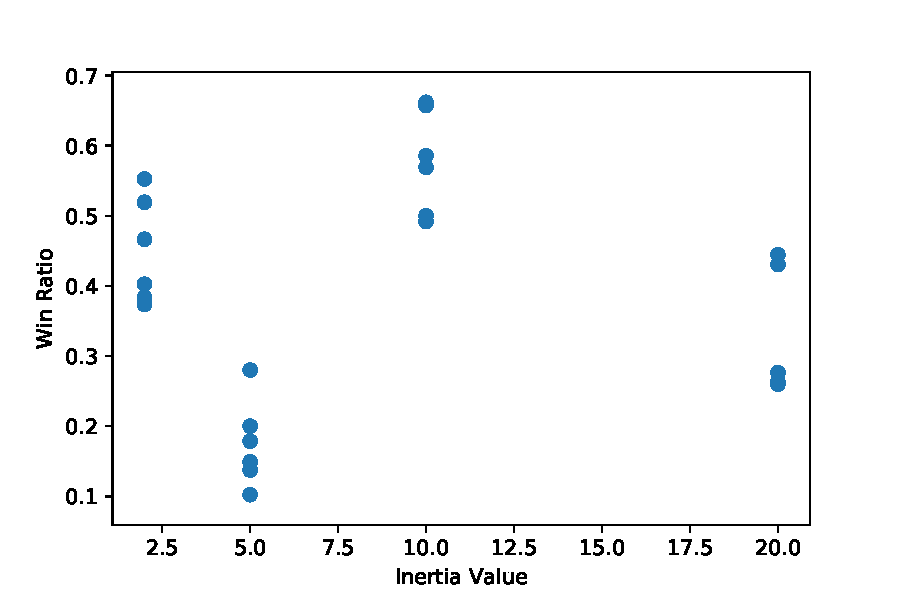
\includegraphics[width=\linewidth]{WinRatioAgainstInertia.pdf}
	\caption{PSC win Ratio against inertia.}
	\label{fig:WinRatioAgainstInertia}
\end{figure}

Inertia was added to PSC due to a need to sustain a consistent strategy and avoid units jumping between actions. This requires a significantly high value as otherwise this issue would persist, however too large  a value would negate the real-time strategy choosing element of the agent. The validated value of 10 seems appropriate to hold a strategy, as the game state will not be amended too drastically and the initial strategy decision would still be relevant.

\subsubsection{Pathfinding Algorithm}

We tested 2 different algorithms, AStarPathFinding and BFSPathFinding. Due to time constraints, we chose a subsection of the algorithms that are found in $\mu$RTS, with these two shown as the most common. The outcomes of this test can be shown in figure \ref{fig:WinRatioAgainstPathfinding}, with the strongest result being shown to be A* PathFinding.

\begin{figure}
	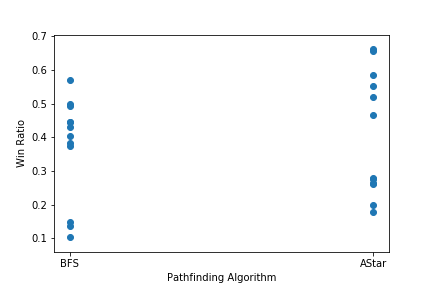
\includegraphics[width=\linewidth]{WinRatioAgainstPathFinding.png}
	\caption{PSC win ratio against pathfinding algorithms.}
	\label{fig:WinRatioAgainstPathfinding}
\end{figure}

A* Pathfinding searches the path space using a heuristic to estimate the distance of a node with respect to the target. A* keeps a list of open nodes and searches the next state with the lowest aggregated distance travelled and distance to the target. This allows the fastest path to be followed, particularly with a perfect distance heuristic function in microRTS. 

\subsubsection{Evaluation Function}

We tested 3 evaluation functions, the provided SimpleSqrtEvaluationFunction3 \&  LanchesterEvaluationFunction and our ComplexEvaluationFunction. We chose these to range from a simple unit comparison to a more in-depth analysis of the positions of each unit relative to the max player. The outcomes of this test can be shown in figure \ref{fig:WinRatioAgainstEvalFunc}, with the highest win ratio using the LanchesterEvaluationFunction.

\begin{figure}
	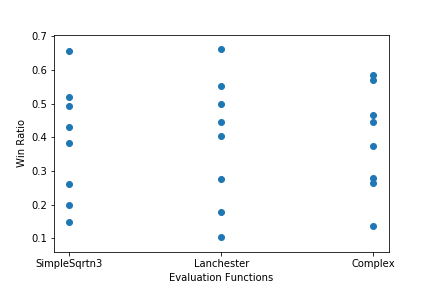
\includegraphics[width=\linewidth]{WinRatioAgainstEvalFunc.png}
	\caption{PSC win ratio against evaluation functions.}
	\label{fig:WinRatioAgainstEvalFunc}
\end{figure}

When analysing the tournament results, it can be seen that none of the tested evaluation functions worked significantly better than the others. Even though we had created the ComplexEvaluationFunction ourselves, this tournament shows how it does not add any benefit. Occam’s Razor states that the simplest proposal is often the best, with less assumptions and speculations. For PSC, we wished to reduce overfitting and not use an overly complicated heuristic measure with no proven benefits. Therefore, we decided to proceed with the simplest evaluation function of SimpleSqrtEvaluationFunction, as it would also be computationally less expensive than its more complex counterparts. 

\subsection{Final Benchmark Tournament}

After we had set our parameters to the optimal found in the validation set, we ran PSC in a final test against a set of complex bots to verify the parameters that we had initialised and provide a final benchmark of the agent. This was conducted with 4 rounds of games on each of the 4 maps that are provided for the competition, totalling to 16 games against each bot.

\begin{table}[]
\caption{wins sc vs bots}
\label{table:bottournament}
\begin{tabular}{llll}
\toprule
Bot       & Win & Lose & Draw\\ \midrule
SCV       & 12  & 2    & 2\\
PortfolioAI & 11  & 5    & 0\\
ABCD    & 16  & 0    & 0  \\
puppet    & 16  & 0    & 0    \\
UCT       & 16  & 0    & 0     \\
Minimax   & 16  & 0    & 0    \\
Naivemcts & 15  & 0    & 1    \\ \bottomrule
\end{tabular}
\label{table:finalbotwins}
\end{table}


Table \ref{table:bottournament} shows the results of this benchmark tournament, with the results being each bot against PSC. Where the scores don't add up to 16, draws had occurred between the bots.
This shows that we conclusively beat a large range of bots on each map, with only PortfolioAI (66\% win ratio) \& SCV (86\% win ratio) winning any games against PSC. This result confirms that our parameters have been maximised for winning and provides a strong confidence that our bot will perform well in the competition.







\section{Analysis}

Portfolio planning is an approach that has been shown to be effective in RTS games \cite{churchill2013portfolio}. It chooses a global strategy based on the current circumstances as opposed to rigidly following a hard-coded strategy. PSC was designed to adapt this portfolio planning model, incorporating elements of domain knowledge and adding the inertia parameter. As can be seen with our final win ratio of 66\% over Portfolio AI and significant dominance over other agents, PSC outperforms the competition provided in $\mu$RTS.

As PortfolioAI is the only bot that remains a challenge to PSC, win ratios against it have become the main measure of the strength of PSC. This is because PSC had 100\% win ratio against other AIs, therefore small improvements or detriments in the performance were unmeasurable against them. It may have been possible to use these AIs if the variation in maps had been greater, but it would have required a large number of maps to notice this affect and the validation time would have increased greatly as a result.

Using the win ratio against PortfolioAI as the performance metric presented some problems; Once we start to win against PortfolioAI, how do we continue to measure and improve it? A win ratio of 100\% against all existing AI does not suggest a perfect bot. PortfolioAI works at a higher level than most other $\mu$RTS agents and so we cannot be sure that PSC’s parameters are simply well trained to counteract PortfolioAI. We will only be able to confirm this with another competitive AI that PSC might be vulnerable to. 

To provide more meaningful competitors to PSC, human players could be incorporated. Due to the human ability to see the global scale and strategy of the game, decisions would be made proactively as opposed to reactively. This would give a proper challenge to the agent, so we can gain more confidence in agent performance and benchmark the results. However, running tests against humans is time consuming, provides inconsistent results and it would not be repeatable for future work.

Even though we are moving towards a more fluid strategy decision, PSC is still relatively hard-coded due to its lack of long-term learning. Further work could be conducted into incorporating a learning element into the agent, potentially leading to a General Adversarial Network approach of playing PSC against itself to learn, similar to work done with AlphaGo Zero \cite{silver2017mastering}. 

Looking at our experimental results, it can be seen that different evaluation functions work well with different inertias. This shows that there is a non-convex relationship between the three validated parameters; inertia, pathfinding and evaluation function. The grid search method of testing these parameters can conclusively determine the best combination, analysing the agent as a whole rather than separate parts.

During validation the optimal inertia parameter, $I$ was found to be 10, justifying the inclusion of inertia within the agent. We were surprised by the inertia approach working so effectively, due to the slight departure from the main look-ahead search approach of portfolio planning. This was a later introduction into the algorithm, as we were seeing the agent perform weakly against a continuous strategy like WorkerRush or LightRush. The experiments now show our superiority over these bots, further justifying the inclusion of the inertia parameter. 

We saw that an $I$ of 20 reduced win ratio, highlighting a trade off between regularity of decisions and depth of search for simulations. Intuitively we can see this as the agent ‘overthinking’ the problem. We only tested $I$ as 2,5,10 \& 20 and saw a local maxima at 10, but did not explore the search space around this. Future work could look at expanding this by testing on smaller increments

Tuning the PathFinding Algorithm and Evaluation Function parameters are ways to optimise the performance of our agent rather than inherently changing its approach. These have been tuned to the optimal value, of A* PathFinding and the SimpleSqrtEvaluationFunction. Pathfinding is an important part of every hardcoded strategy employed by PSC, which justifies the large increase in game success with an effective function.

The main difficulty with applying PSC, or any look-ahead search technique, to a RTS game like $\mu$RTS, is the lack of an effective evaluation functions. These RTS games do not have an explicit reward function apart from the terminal end scoring, which often is too far down the simulation space to reach. Even though the varying evaluation functions we propose do not have a significant effect on the tournament results, we believe a robust evaluation procedure would greatly improve performance, with the ability to evaluate the simulated game an underpinning element of our agent.
 
Our agent was tested in the $\mu$RTS game, but could be expanded for larger RTS games like StarCraft and Dota. However, our experiments within microRTS were conducted against current built-in AIs which are weaker opponents than current state-of-the-art bots. As the larger games have more complex actions and extensive branching factors, it would not be conclusive to say our success in $\mu$RTS would be repeated. As Portfolio Greedy Search is only used in combat situations within StarCraft, we expect the PSC agent could be similarly applied to deal with small parts of the overall StarCraft strategy \cite{churchill2013portfolio}.

\section{Conclusions}


In this paper, we have described an agent for playing the $\mu$RTS game called Portfolio Strategy Chooser, which is a strategy abstraction mechanism based on greedily searching the simulated state space to evaluate global strategies. This takes into account the short thinking time of 100ms available and the large branching factor of the game, motivating a simulation-based approach. We have shown that PSC outperforms PortfolioAI consistently, with a win ratio of 66\% and a strong dominance over other agents.


\subsection{Future work}
 

There could be future work in evaluating a larger bucket of strategies, simulating a small amount and pruning those that are not promising, allowing a larger simulation time for the hopeful strategies. The prediction of enemy strategies could also be enhanced by deeper analysis of the enemy player, potentially analysing the opponents past moves, allowing a more accurate simulation. 

Further decision rollouts could be included in the search tree to improve the accuracy of the evaluation. Currently, Portfolio Strategy Chooser optimises only the decision at the root node of the tree before performing its playout evaluation. By expanding this to look further down the tree to moves in the future, a hybrid tree search algorithm could be imagined, in which PSC is the method used by a minimax type algorithm to choose which moves to play at a given node in the tree.

Improvements could also be made to the evaluation function, taking a large data source of previous game states and final outcomes and using deep learning to understand which states are best placed for success. This would follow on from the success of AlphaGo to analyse a current game board and return an effective evaluation score \cite{silver2016mastering}. Deep Convolutional Neural Networks could be utilised in the same vein, taking a snapshot of the current game state and returning an evaluation score, following on from work done in $\mu$RTS\cite{barriga2017combining}.

\bibliographystyle{unsrt}
\bibliography{bibliography.bib}

\end{document}
